\section{Results}\label{sec:results}
The specification uses a triple-difference interpretation. The three differences are: (i) between pre- and post-treatment periods, (ii) between tariffed and non-tariffed products, and (iii) between deep and non-deep trade agreement countries. This design allows me to examine whether trade agreement depth moderates the effect of tariffs on import prices. As formalized by \textcite{oldenTripleDifferenceEstimator2022}, valid triple-difference interpretation requires that the relative performance of tariffed versus non-tariffed products be similar across deep and non-deep countries prior to treatment. This assumption is addressed throughout this section. 

\subsection{Sample calibration}

    \begin{figure}[h]
        \centering
        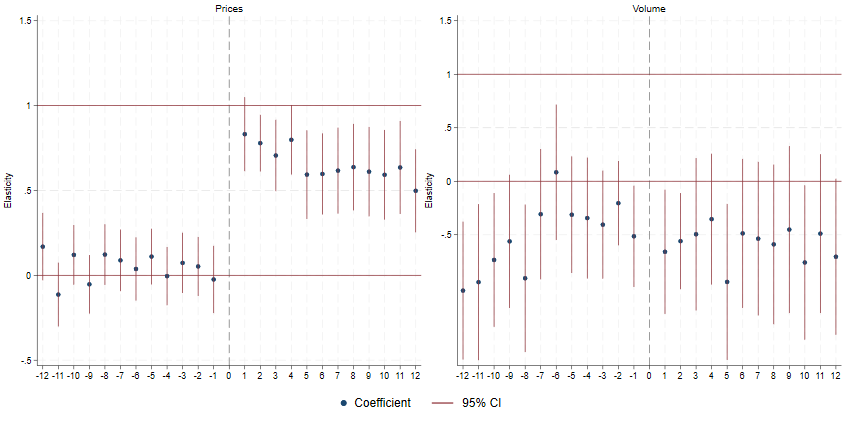
\includegraphics[width=0.85\linewidth]{../Figures/reg_figures/reg_baseline_combined.png}
        \caption{Sample calibration regression results}
        \label{fig:sample_calibration}
    \end{figure}

As seen in Figure~\ref{fig:sample_calibration}, the restricted sample's prices behave similarly to the complete pass-through found in \textcite{amiti_whos_2020}. In contrast to the universal sample's sustained and steady complete pass-through, it appears that within this sample, pass-through approached one initially before declining to approximately 0.5. This is most consistent with Amiti's findings for steel inputs, which show steel prices to follow a nearly identical pattern with minor variations. Pre-trends, meanwhile, are statistically indistinguishable from zero, indicating zero pre-trends are likely. This was also the case in Amiti's sample --- both universal and specific to steel. 

Volumes exhibit some pre-trends, with volume elasticity rising slightly before stabilizing over -0.5 at 6 months before treatment. Following treatment, we see no meaningful change, but for a slight increase in the four months after tariff implementation and a subsequent noisy decline. Overall, confidence intervals are wide and steadily occupy roughly the same area, between approximately 0 and -1. The results in \textcite{amiti_whos_2020} exhibit a small negative but rising volume elasticity between 12 and 6 months prior to treatment, before steadily declining across the board following tariff implementation. Steel products experienced the smallest negative elasticity, never reaching far below -1. This roughly matches the restricted sample, though the sample's post-treatment outcomes are less clearly identified. 

This sample suggests that tariffs saw incomplete pass-through of tariffs to prices, with a minimal effect on volumes. Of the categories and product types examined in \textcite{amiti_whos_2020}, these trends most closely resemble those of the steel category studied in \textcite{amiti_whos_2020}.\footnote{These charts are available in \autocite{amiti_whos_2020}.}  

\subsection{Differential agreement effect}

    \begin{figure}[H]
        \centering
        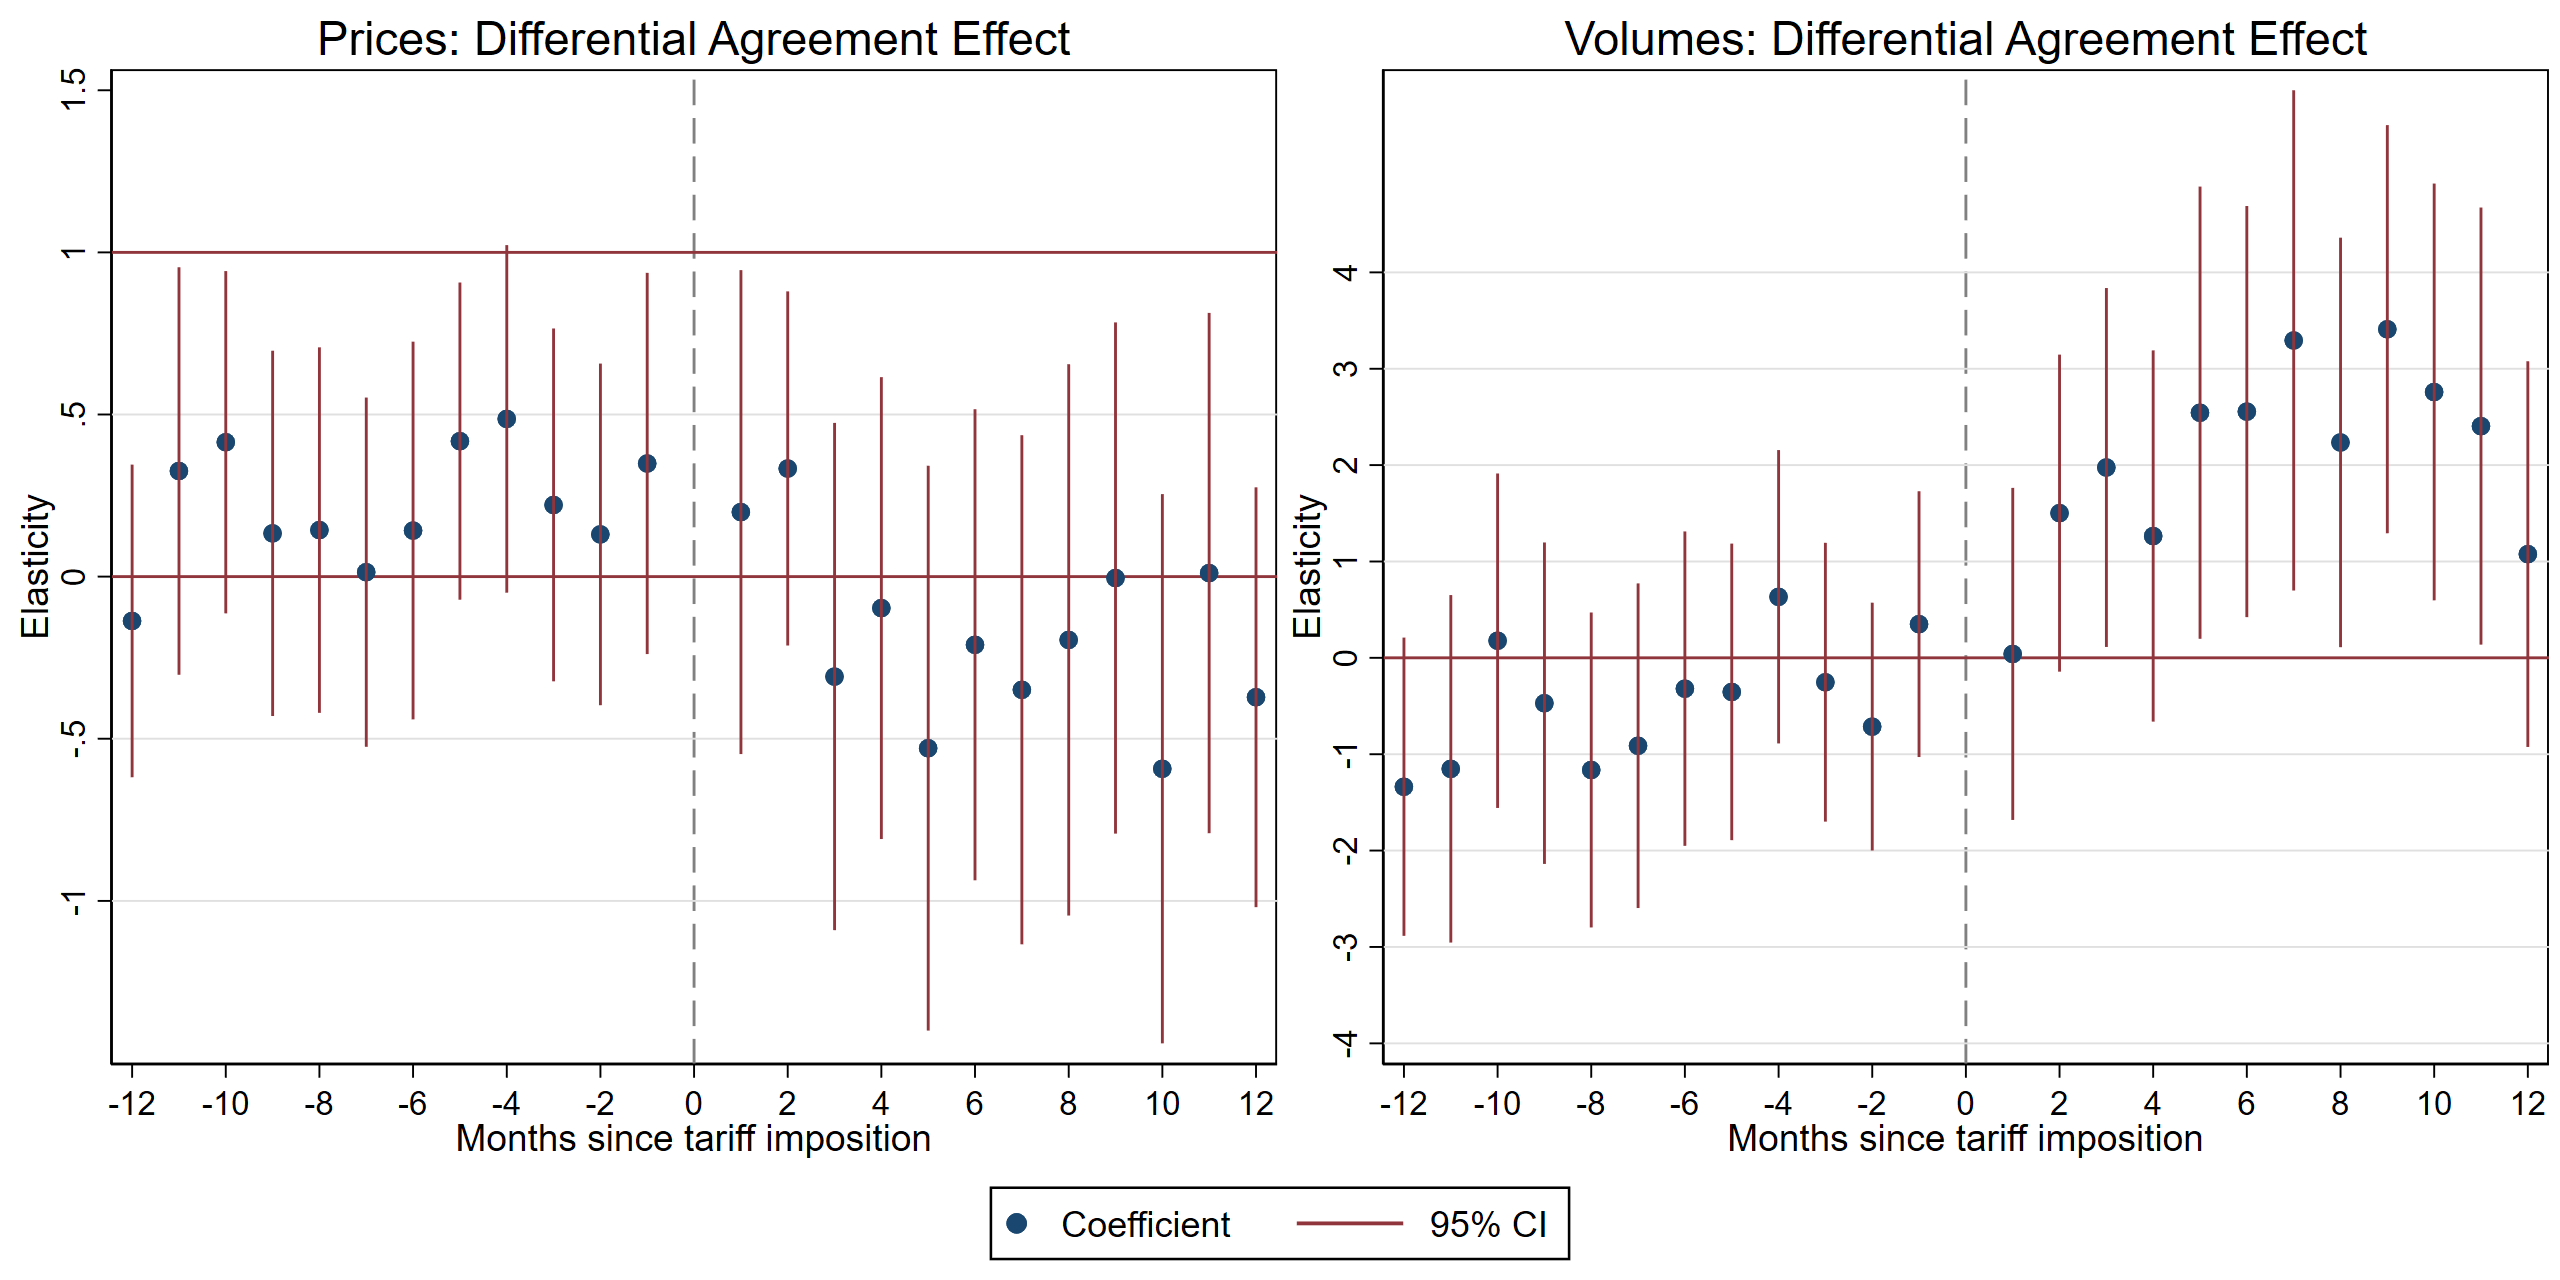
\includegraphics[width=0.85\linewidth]{../Figures/reg_figures/reg_all_diff_combined.png}
        \caption{Agreement vs No agreement regression differences}
        \label{fig:reg_all_diff_combined}
    \end{figure}

The differential effect of trade agreements on prices and volumes is identified by computing the difference between the coefficients for the subsample of countries with bilateral trade agreements and those for the subsample of countries without bilateral trade agreements with the US. These differential outcomes exhibit markedly different patterns than the above regression. The panels in Figure~\ref{fig:reg_all_diff_combined} show the estimated differential monthly elasticities of tariff-inclusive import prices and import volumes for 12 months before and after treatment. While a null effect of trade agreements would require the monthly coefficients to equal zero in both panels, this is evidently not the case.

On the surface, the results suggest that agreement countries experienced smaller price pass-through and a relative increase in import volumes compared to non-agreement countries. Because these coefficients reflect differential effects between the two groups rather than absolute responses, further analysis is required to interpret what they reveal about the effect of tariffs on prices and volumes. Nonetheless, the patterns are consistent with the initial hypothesis that trade flows between the US and its agreement partners would prove more resilient to unilateral tariff shocks.

The differential effect of tariffs on prices for countries with versus without bilateral trade agreements with the US is shown in Figure~\ref{fig:reg_all_diff_combined}. Pre-treatment differential coefficients are consistently positive, though mostly small in magnitude, and statistically indistinguishable from zero in most months, satisfying the parallel trends assumption. Following tariff implementation, the differential remains positive for two months --- in line with pre-treatment coefficients --- before turning negative, where it remains through the rest of the post-treatment window. On the surface, this pattern suggests a delayed moderating effect of trade agreements on tariff pass-through.

The underlying agreement-status regressions in Figure~\ref{fig:reg_all_agrstatus_combined} clarify what is driving this differential. Panel (1) shows that agreement countries experienced a sharp price increase in the first two months following tariff implementation --- larger than the corresponding response in non-agreement countries (panel (2)) --- before settling to a price elasticity slightly below the non-agreement group in subsequent months. What appeared on the surface to be a delayed moderating effect was in fact elevated initial pass-through followed by partial absorption. Although the data is noisy, the consistently negative differential in the medium term indicates that trade agreements have a slightly moderating effect on tariff pass-through to border prices. Section~\ref{sec:interpretation} discusses possible mechanisms.

    \begin{figure}
        \centering
        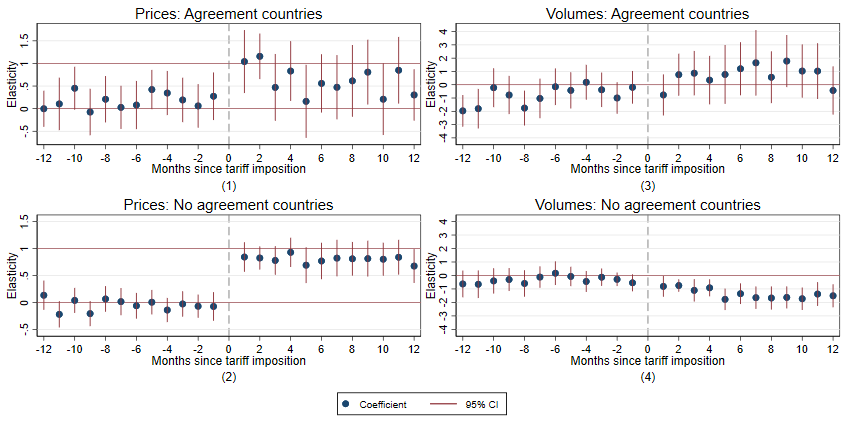
\includegraphics[width=0.85\linewidth]{../Figures/reg_figures/reg_all_agrstatus_combined.png}
        \caption{Agreement vs No agreement regression results}
        \label{fig:reg_all_agrstatus_combined}
    \end{figure}
    
The differential effect of tariffs on volumes (Figure~\ref{fig:reg_all_diff_combined}) exhibits a starker and clearer pattern. Pre-treatment coefficients are statistically insignificant at the 5\% level, indicating no evidence of relative pre-trends. Following tariff implementation, import volumes from agreement countries display substantially higher differential elasticities than non-agreement countries while increasing over time, with the differential ranging from 1 to 3 in most months. Taken at face value, the modal 25\% tariff would --- all else equal --- generate a peak 75\% difference in the volume response between the two groups around eight months after implementation, though wide confidence intervals caution against literal extrapolation. This pattern admits two interpretations: agreement countries may be experiencing a smaller drop in volumes, or an outright rise in volumes while non-agreement countries decline.

Figure~\ref{fig:reg_all_agrstatus_combined} supports the latter. Volumes from agreement countries rise over time (panel (3)), while non-agreement countries' volumes decline steadily for six months following tariff implementation before plateauing at an elasticity slightly above $-2$ (panel (4)). This implies that a 25\% tariff would generate an approximately 44\% decline in imports from non-agreement countries twelve months after implementation, while producing an approximately 25\% rise in imports from agreement countries.

Taken together, the aggregate results indicate that bilateral trade agreements with the US moderate the effects of tariffs on both  prices and volumes, with the volume response substantially clearer than the price response. Agreement countries experience higher initial pass-through that gradually transitions to partial absorption, while their import volumes rise even as non-agreement countries see import volumes fall. These patterns are consistent with the hypothesis that institutionalized trade relationships provide some resilience to unilateral tariff shocks. However, the aggregate sample combines steel and non-steel products, and the close resemblance of these results to the steel-only patterns reported in \autocite{amiti_whos_2020} raises the possibility that steel products, which constitute the majority of the sample, are driving the aggregate findings. Section~\ref{sec:steel_heterogeneity_results} examines whether the differential agreement effect holds within each product category separately.

\subsection{Triple-difference by steel and non-steel products}\label{sec:steel_heterogeneity_results}

\begin{table}[H]
\centering
\caption{Sample decomposition (count of country-product pair)}\label{tab:steel_share}
    \begin{tabular}{c | cc | c}
    \hline
    & \textbf{Steel} & \textbf{Non-steel} & \textbf{Total} \\
    \hline 
                \textbf{Agreement} & 35,130 & 16,262 & 51,392 \\
                & 14.1\% & 6.5\% & 20.6\% \\

                \textbf{No agreement} & 126,196 & 72,535 & 197,731 \\
                & 50.7\% & 29.1\% & 79.8\% \\
            \hline
                \textbf{Total} & 161,326 & 87,897 & 249,123 \\
                & 64.8\% & 35.3\% & 100\% \\        
    \end{tabular}
\end{table}

Table~\ref{tab:steel_share} decomposes the sample by steel and non-steel products, revealing that steel products constitute nearly 65\% of the country-product pairs and 68\% of the agreement subsample.\footnote{Calculation: $14.1\% / 20.6\% = 68.4\%$.} This composition raises two related concerns. First, the close resemblance of the aggregate results to the steel-only patterns reported in \autocite{amiti_whos_2020} could simply reflect that steel observations dominate the aggregate by construction. Second, and more substantively, the differential agreement effect may operate differently across product categories, and the aggregate result could mask meaningful heterogeneity. To distinguish these possibilities, I implement Equation~\ref{eq:heterogeneity} with $B \in \{\textnormal{steel}, \textnormal{non-steel}\}$, estimating the differential agreement effect separately within each product category.

\subsubsection{Prices of steel vs. non-steel products}

    % Steel vs non-steel Prices: Differences
    \begin{figure}[H]
        \centering
        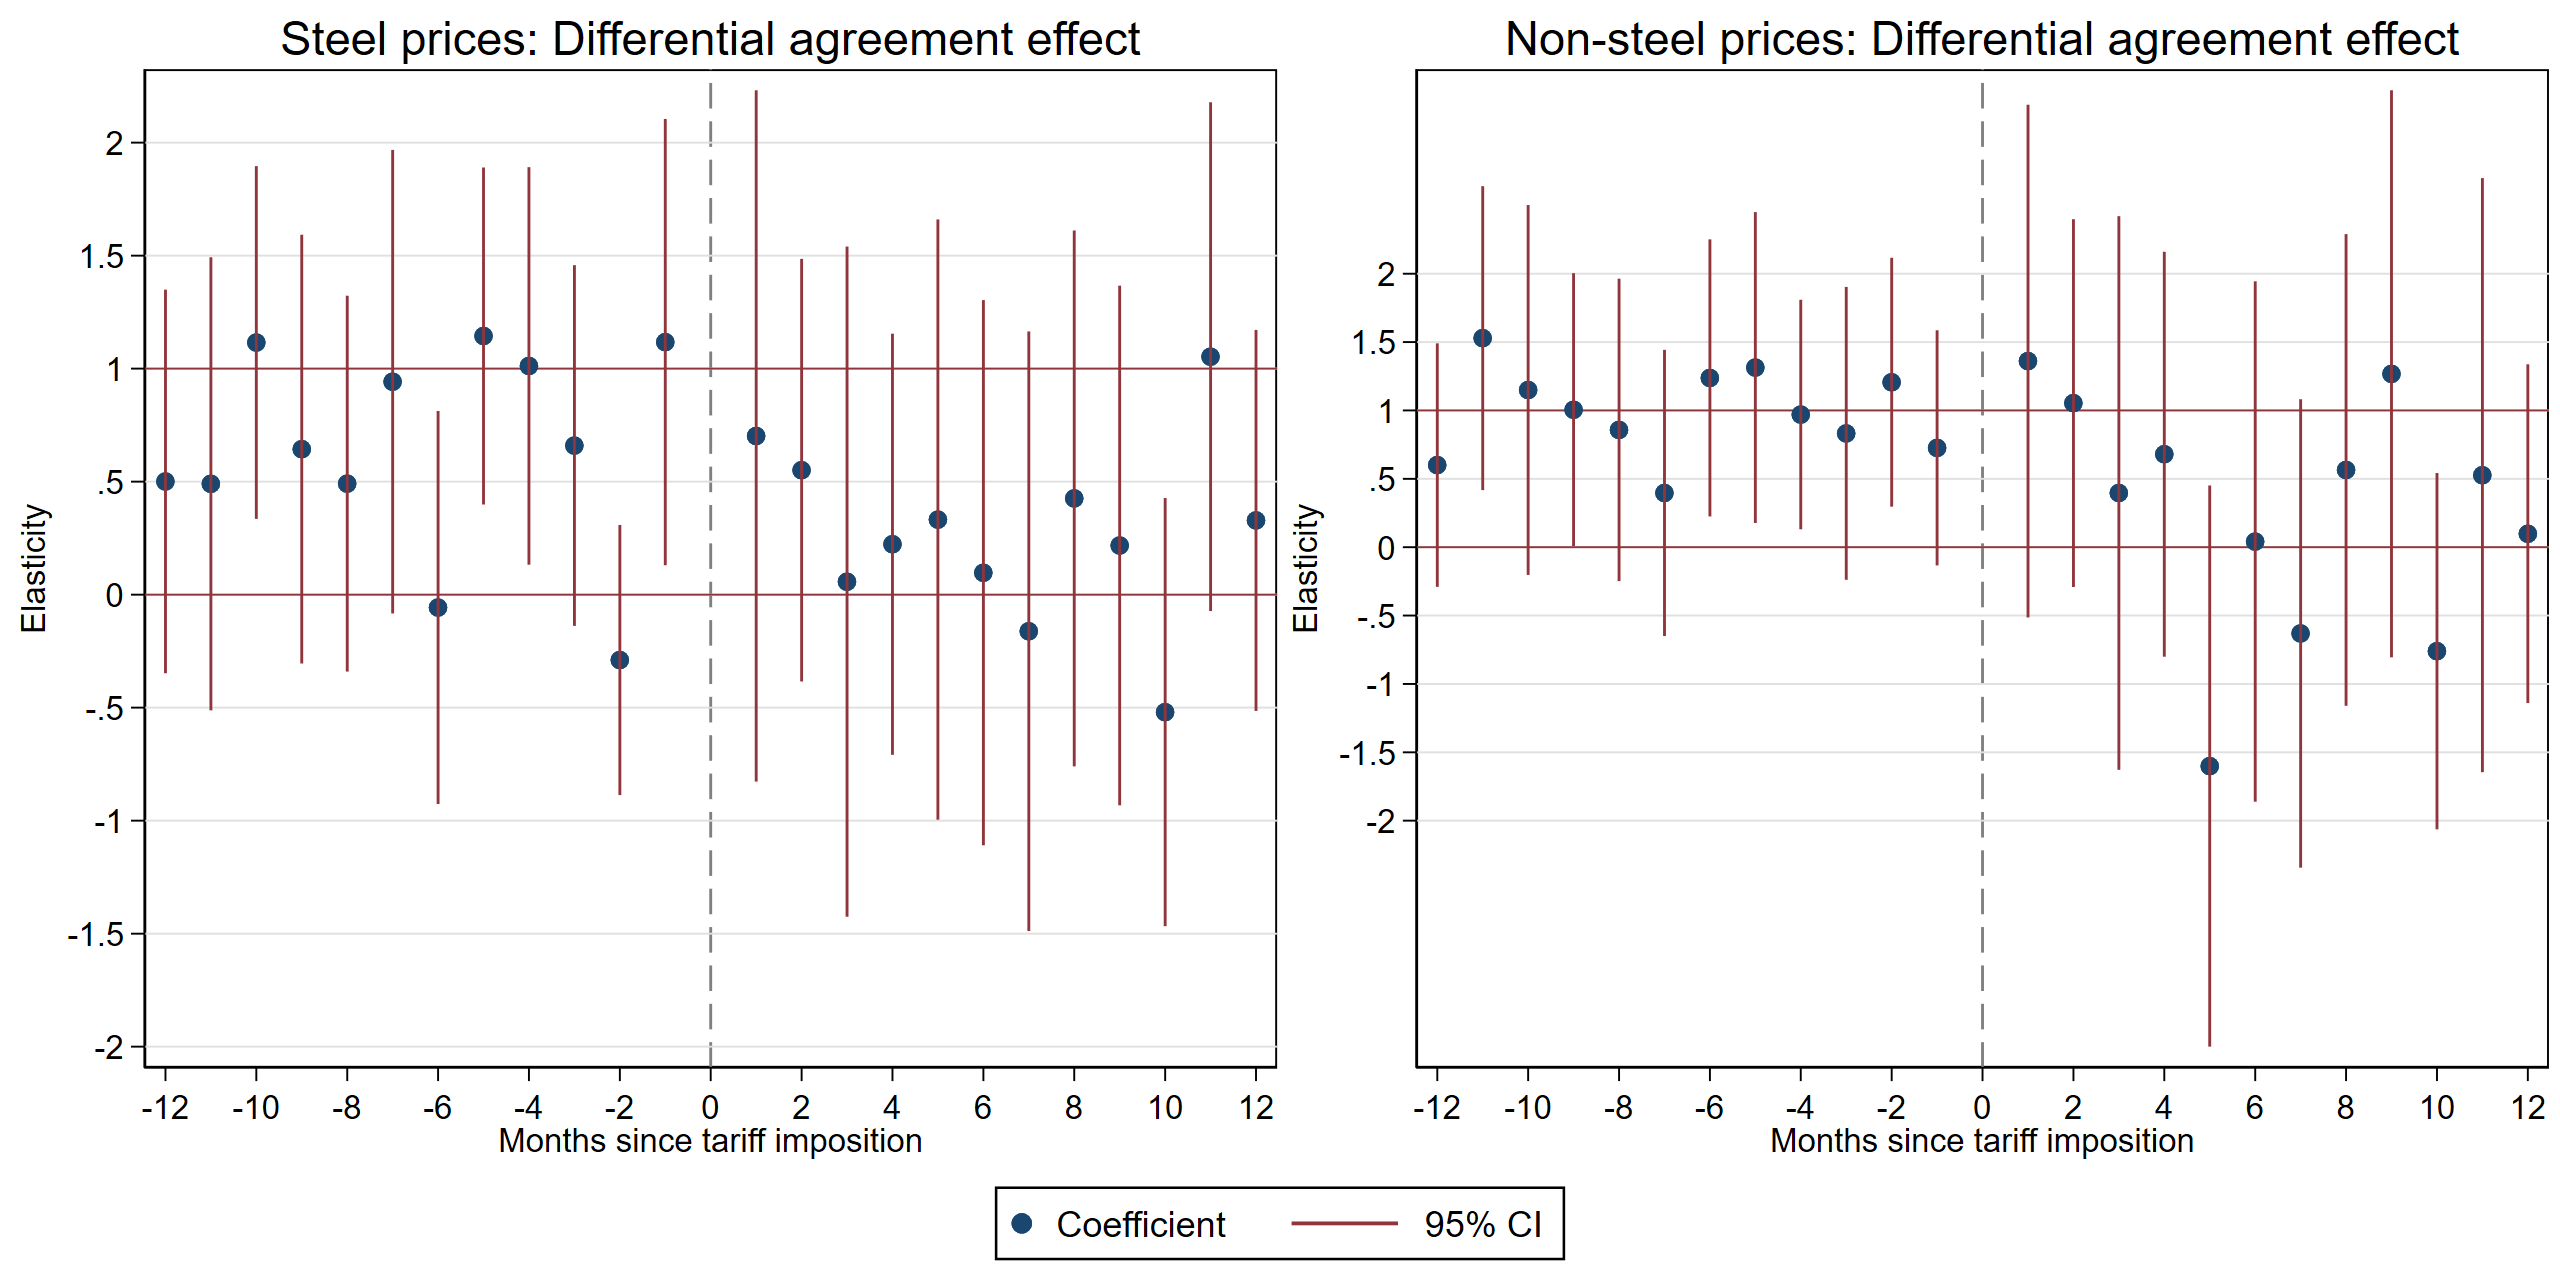
\includegraphics[width=0.85\linewidth]{../Figures/reg_figures/steel_prices_diff.png}
        \caption{Steel vs non-steel prices: Differential effect of agreements}
        \label{fig:steel_prices_diff}
    \end{figure}

    % Steel vs non-steel Prices: By agreement status
    \begin{figure}[H]
        \centering
        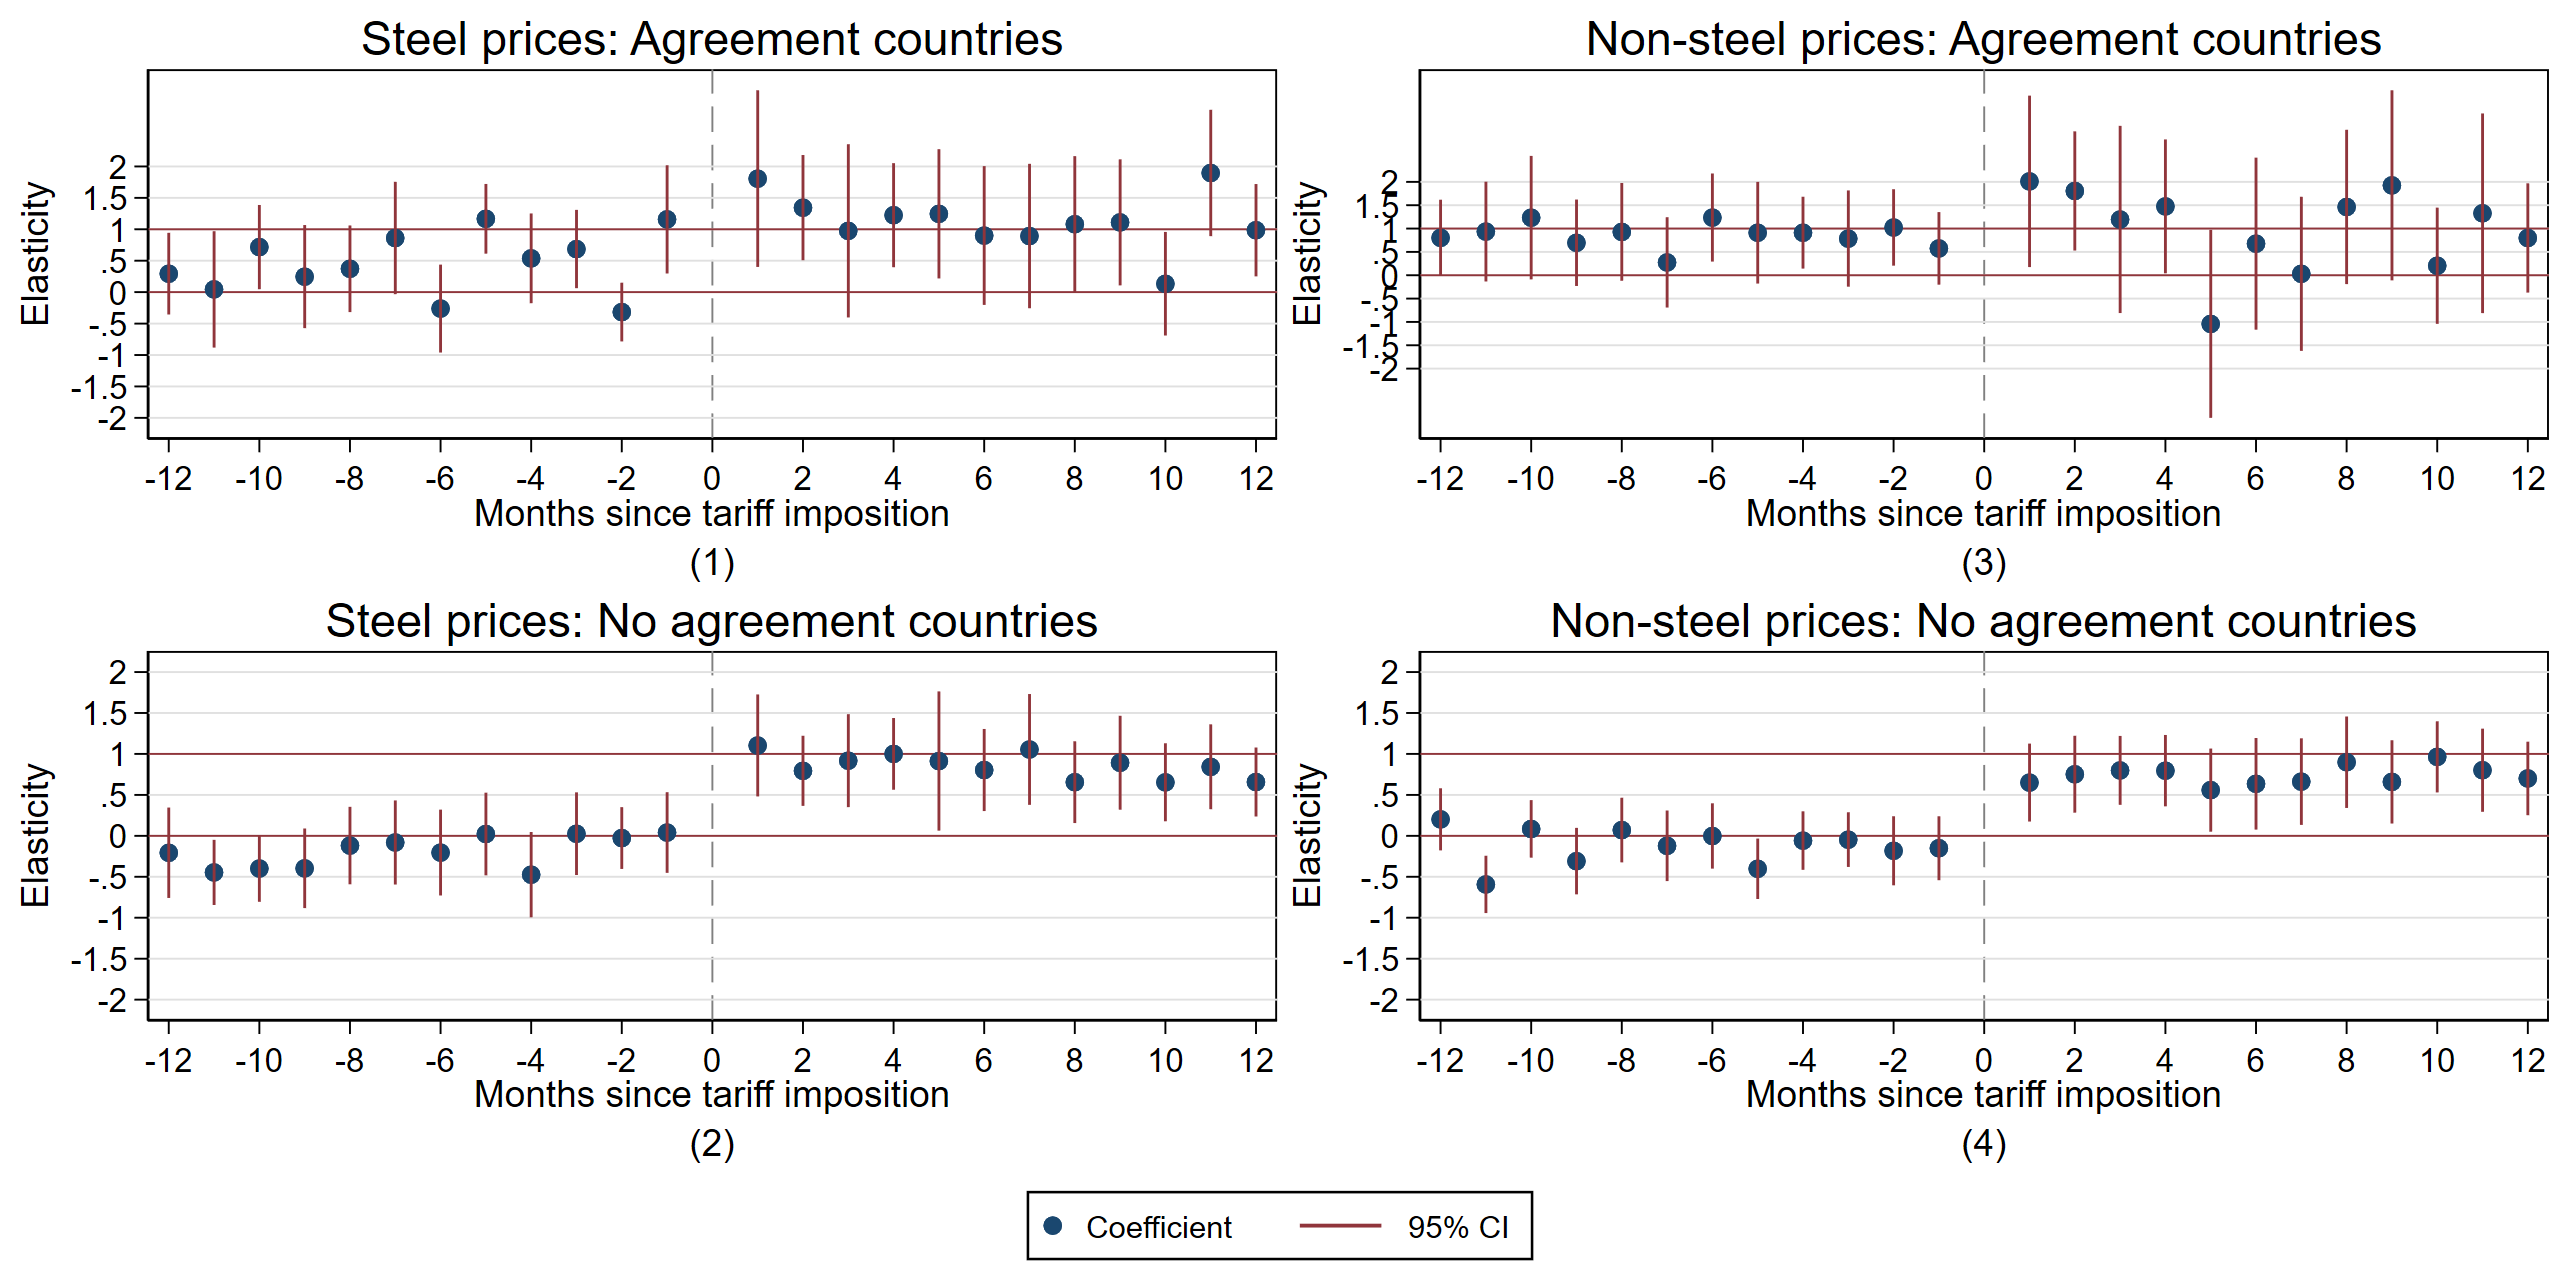
\includegraphics[width=0.85\linewidth]{../Figures/reg_figures/steel_prices_agrstatus.png}
        \caption{Steel vs non-steel prices: Regressions by agreement status}
        \label{fig:steel_prices_agrstatus}
    \end{figure}

Two comparisons help assess whether steel observations dominate the aggregate result. First, comparing the aggregate differential effect (Figure~\ref{fig:reg_all_diff_combined}) to the steel and non-steel differentials (Figure~\ref{fig:steel_prices_diff}) reveals some post-treatment similarity between the aggregate and steel patterns, but substantial differences elsewhere. Both subsample differentials exhibit noisy pre-treatment coefficients with seemingly positive pre-treatment price elasticities, in contrast to the cleaner, nearly null pre-trends in the aggregate. The post-treatment patterns also diverge: while the aggregate differential settles into a consistently negative band, the steel and non-steel differentials are more volatile and less precise. Second, comparing the agreement and non-agreement split-sample regressions across the aggregate (Figure~\ref{fig:reg_all_agrstatus_combined}) and the product-category subsamples (Figure~\ref{fig:steel_prices_agrstatus}) shows that within each agreement-status group, the steel and non-steel coefficients appear statistically indistinguishable based on overlapping confidence intervals. 

Together, these comparisons suggest that the differential agreement effect is not mechanically driven by the steel-heavy composition of the aggregate sample. Although steel observations constitute the majority of the data, the steel and non-steel subsamples do not exhibit meaningfully different differential agreement effects, and the aggregate result appears to reflect a pattern that holds across both product categories rather than one driven by steel alone. The pre-trend concerns raised by the subsample comparisons, however, warrant closer examination, which the following analysis addresses.

Figures~\ref{fig:steel_prices_agrstatus} and \ref{fig:steel_prices_diff} reveal a pre-trend violation that undermines causal interpretation of the agreement differential with respect to prices. Within both steel (Fig. \ref{fig:steel_prices_agrstatus} (1)) and non-steel (Fig. \ref{fig:steel_prices_agrstatus} (3)) products, agreement countries exhibit systematically positive pre-treatment price coefficients while non-agreement countries display null pre-trends (Fig. \ref{fig:steel_prices_agrstatus} (1) and (3)), generating a positive agreement/non-agreement differential prior to tariff implementation. Since all coefficients are defined relative to the last pre-treatment month, these positive pre-period coefficients imply the differential was elevated in earlier months and declined into the baseline, before recovering post-treatment. This pattern is inconsistent with the parallel trends assumption required for causal identification of price elasticity in this context: the differential was already moving before tariffs were imposed, and post-treatment estimates cannot be cleanly attributed to tariff pass-through heterogeneity by whether or not countries have trade agreements with the United States. One source of this instability could be heterogeneity between steel products sourced from countries with versus  without trading agreements, coupled with a smaller set of countries within the agreement subsample. Steel and non-steel products from countries with US trade agreements may fundamentally be different from global products, resulting in some pre-trends. As a result, the product-time fixed effect $\delta_{jt}$ may be absorbing fundamentally different variation that explains the discrepancy. Another could be that perhaps the pre-treatment month is anomalous in some way, perhaps due to anticipation of tariffs. 

Accounting for the fact that there may be some distortion in the pre-treatment sample, it does appear that for both steel and non-steel products, there is some effect of tariffs within imports from countries with trade agreements. Elasticity for steel products from this group of countries (Fig. \ref{fig:steel_prices_agrstatus} (1)) fluctuates between 0 and 1 before tariff implementation, but rises afterwards. Once tariffs are imposed, elasticity jumps to about 2 before declining to a tight band around 1. In any case, there is a clear difference --- taking the approximately 0.5 elasticity pre-treatment coefficients hover around at face value, it seems there is an increase in pass-through due to tariffs within this group to the magnitude of approximately 0.5 relative to the pre-treatment elasticity. Comparing this directly to the effect of tariffs on steel prices within the non-agreement group, it appears that agreement countries experienced a slightly smaller increase in price elasticities following tariffs' imposition. Based on this comparison of pre- and post-treatment elasticities, it appears that in fact, countries with trade agreements did indeed have lower pass-through than agreement countries. This cannot be interpreted causally, however, due to the major violation of the zero relative pre-trends assumption. 

This pattern is replicated in non-steel products. While pre-treatment elasticities are elevated around 1 for agreement countries, they rise to 2 immediately after tariffs are imposed before declining over the first quarter. Following this, elasticities fluctuate dramatically. While this is likely a result of the small sample size for non-steel country-product pairs where the country has a trade agreement with the US (N=16,262), the difference between the pre-treatment and post-treatment elasticities for agreement countries appears once again to be slightly smaller on average than for non-agreement countries. Meanwhile, this volatility is notable, particularly as the coefficients remained in a relatively narrow band before implementation. This fluctuation suggests there could be a high degree of heterogeneity within this subsample in how foreign exporters respond to tariffs. 

\subsubsection{Volume of steel vs. non-steel products}

    % Steel vs non-steel Volume: Differences
    \begin{figure}[H]
        \centering
        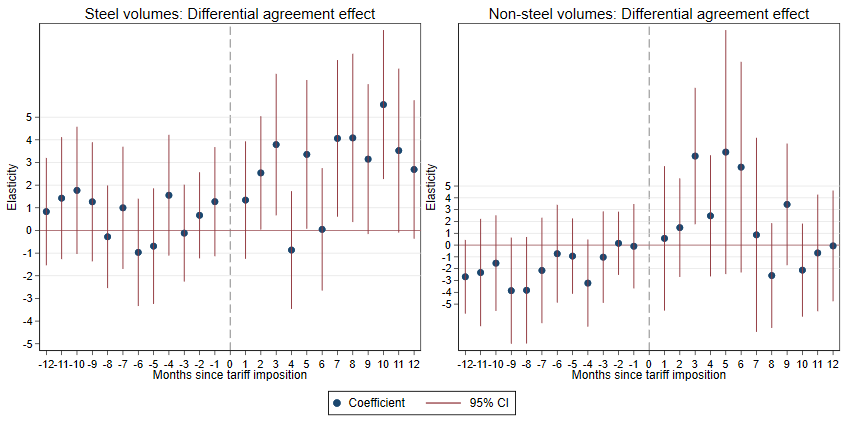
\includegraphics[width=0.85\linewidth]{../Figures/reg_figures/steel_volume_diff.png}
        \caption{Steel vs non-steel volumes: Differential effect of agreements}
        \label{fig:steel_volume_diff}
    \end{figure}

    % Steel vs non-steel Volume: By agreement status
    \begin{figure}[H]
        \centering
        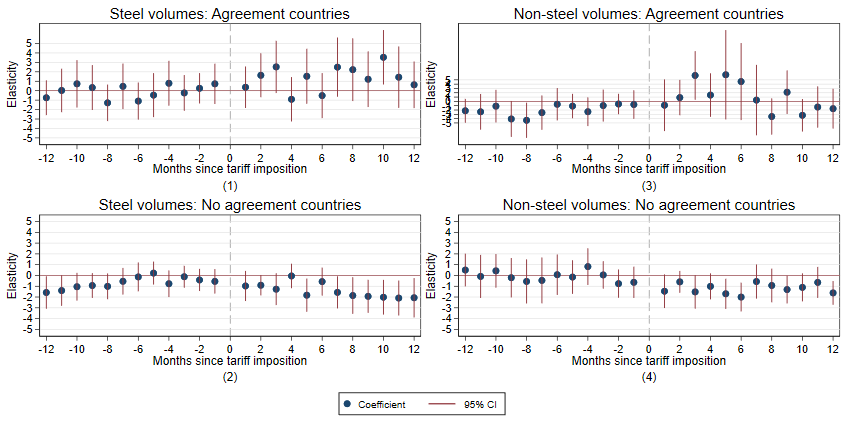
\includegraphics[width=0.85\linewidth]{../Figures/reg_figures/steel_volume_agrstatus.png}
        \caption{Steel vs non-steel volumes: Regressions by agreement status}
        \label{fig:steel_volume_agrstatus}
    \end{figure}

To assess whether the differential effect of agreements on volume elasticities is driven by the dominant steel subsample, I repeat the same exercise as above. First, comparing the aggregate differential (Figure~\ref{fig:reg_all_diff_combined}) to the steel and non-steel differentials (Figure~\ref{fig:steel_volume_diff}), the steel differential closely resembles the aggregate, while the non-steel differential is broadly similar in the first six post-treatment months before diverging substantially after seven months. Second, examining the agreement and non-agreement split samples within each product category (Figure~\ref{fig:steel_volume_agrstatus}) reveals that within the non-agreement group, steel and non-steel exhibit similar volume elasticities and both resemble the aggregate non-agreement pattern. Within the agreement group, however, the steel and aggregate patterns align, while the non-steel pattern diverges after seven months post-tariff implementation, dropping into negative elasticity territory.

This decomposition suggests that the steel subsample does drive the aggregate agreement-country result. The aggregate increase in volume elasticities observed for agreement countries reflects the steel-specific pattern, while non-steel agreement-country volume elasticities follow an initially positive trajectory before turning negative. The non-agreement results, by contrast, are consistent across product categories and are not subject to this concern. The divergence between steel and non-steel within the agreement group warrants closer examination, which the following analysis addresses.

Turning to the identification of a differential agreement effect on volume elasticities, the coefficients exhibit clean pre-treatment behavior, in contrast to the ambiguous pre-trends in the price specification. Figure~\ref{fig:steel_volume_diff} shows that the differential volume elasticity is statistically indistinguishable from zero in the pre-treatment period for both steel and non-steel products, satisfying the parallel trends requirement for causal identification of $\beta_s$. Within steel products, agreement countries display a null pre-trend, while non-agreement countries show a slight positive movement between 12 and 6 months prior to treatment (Fig.~\ref{fig:steel_volume_agrstatus}, panels (1) and (2)); this minor deviation does not translate into a meaningful differential, which remains null throughout the pre-period. Within non-steel products, the differential exhibits a slight upward drift, driven by a small positive pre-trend in agreement countries and a small negative pre-trend in non-agreement countries (Fig.~\ref{fig:steel_volume_agrstatus}, panels (3) and (4)). Both group-specific pre-trends remain statistically insignificant in nearly all pre-treatment months, and the differential itself is statistically indistinguishable from zero across both groups. Taken together, the volume specification provides a substantially stronger basis for causal interpretation than the price specification.

Following tariff implementation, the differential volume elasticity is positive for both steel and non-steel products, indicating that agreement countries captured import volume relative to non-agreement countries (Fig.~\ref{fig:steel_volume_diff}). Within steel products, this differential is driven by a large and slightly increasing positive volume elasticity in agreement countries, paired with a negative elasticity in non-agreement countries that fluctuates around $-1$ in the first few post-tariff months before declining further to roughly $-2$ (Fig.~\ref{fig:steel_volume_agrstatus}, panels (1) and (2)). Within non-steel products, the differential is highly positive in the first six months before declining, though all but one month is statistically insignificant (Fig.~\ref{fig:steel_volume_diff}). The agreement-country volume elasticity peaks at approximately 6 around five months post-treatment --- a magnitude that, taken at face value, would imply a $25\%$ tariff generates a $150\%$ increase in import volumes, though the wide confidence intervals at this time horizon caution against literal interpretation. The elasticity subsequently declines, crossing into negative territory after seven months with one outlier, though most post-treatment estimates remain statistically insignificant. By contrast, non-agreement countries exhibit consistently negative non-steel volume elasticities, ranging between $-0.5$ and $-2$ with an average near $-1$, and these estimates are statistically significant in most periods (Fig.~\ref{fig:steel_volume_agrstatus}, panels (3) and (4)).

Taken together, these two exercises reveal that while the subsample is cleanly interpretable with parallel trends satisfied across both product categories, it is not well-balanced. The differential agreement effect on volumes is positive following tariff implementation, indicating that agreement countries captured import share as non-agreement countries lost it. However, this aggregate finding masks heterogeneity: steel products from agreement countries exhibit a large and persistent volume increase, while non-steel products from agreement countries reveal a transient gain that reverses after around six months. Meanwhile, both product categories exhibit consistent volume declines for non-agreement countries. The persistence of the steel trend and the reversal of the non-steel trend suggest that the resilience conferred by trade agreements is product-specific. Coupled with the fact that the first exercise indicates the aggregate sample is dominated by the steel subsample, the model's aggregate findings cannot be interpreted as universal effects, but must be examined at the product level. Section~\ref{sec:interpretation} discusses these mechanisms in light of both the steel and non-steel evidence.

